%!TEX TS-program = xelatex
%!TEX encoding = UTF-8 Unicode
\documentclass[12pt,a4paper]{article}
\usepackage{geometry} % 設定邊界
\geometry{
  top=1in,
  inner=1in,
  outer=1in,
  bottom=1in,
  headheight=3ex,
  headsep=2ex
}
\usepackage{fontspec} % 允許設定字體
\usepackage{xeCJK} % 分開設置中英文字型
\usepackage{url} % 使用url
\usepackage[colorlinks,
            linkcolor= black]{hyperref}
\setCJKmainfont{LiHei Pro} % 設定中文字型
\setmainfont{Georgia} % 設定英文字型
\setromanfont{Georgia} % 字型
\setmonofont{Courier New}
\linespread{1.2}\selectfont % 行距
\XeTeXlinebreaklocale "zh" % 針對中文自動換行
\XeTeXlinebreakskip = 0pt plus 1pt % 字與字之間加入0pt至1pt的間距,確保左右對整齊
\parindent 0em % 段落縮進
\setlength{\parskip}{20pt} % 段落之間的距離

\title{\huge 物聯網應用與資料分析 Assignment5 - Titanic Predict with Keras} % 設置標題,使用巨大字體
\author{姓名:吳嘉偉\quad 學號:5105056013\quad 日期:2018/6/2} % 設置作者
\date{} % 設置日期
\usepackage{titling}
\setlength{\droptitle}{-8em} % 將標題移動至頁面的上面
\usepackage{listings}

% 設置演算法的灰色底
\usepackage{algorithmic}
\usepackage{color}
\definecolor{algorbgm}{gray}{0.85}
\newcommand{\grayblock}[1]{
\colorbox{algorbgm}{\centering
\begin{minipage}{0.8\textwidth} ~\\[-15pt]#1~\\[-25pt] \end{minipage}}}
% example
%\begin{algorithmic}
%\IF{somebody open the door 1}
%\STATE he gets an apple
%\STATE he gets an key
%\ELSIF{somebody open the door 2}
%\STATE he gets nothing
%\ENDIF
%\end{algorithmic}

% 設置灰底
\usepackage{color}
\usepackage{framed}
\definecolor{shadecolor}{gray}{0.85}
% example
%\begin{shaded}
%java -jar test.jar	
%\end{shaded}

\begin{document}

\clearpage

\maketitle % 顯示標題

\section{目標}
{
\fontsize{14pt}{10pt} % 字型大小14pt,字行間距20pt
\selectfont % 生效
利用Kaggle提供的Titanic資料集,透過Keras分析乘客是否生還。

\section{Prepare Data}
{
\subsection{Create Python File}
建立一個preprocess.py的檔案,把資料集預處理的程式碼邏輯寫在這個地方。

\subsection{Get CSV File Data}
下載網站上面提供的train.csv, test.csv。利用python pandas套件把這兩個檔案讀出來。

\begin{shaded}
\begin{lstlisting}[language=Python]
import pandas as pd

def getData():
  train = pd.read_csv('train.csv')
  test = pd.read_csv('test.csv')
  return train, test

\end{lstlisting}
\end{shaded}

\subsection{Fill Missing Data}
因為我們預計要拿Age, Sex, Pclass這三個欄位來做預測,發現Age是有缺值的。所以利用Age這欄位的平均值填在缺值的欄位上

\begin{shaded}
\begin{lstlisting}[language=Python]
def fillMissing(train, test):
  train.Age = train.Age.fillna(train.Age.mean())
  test.Age = test.Age.fillna(test.Age.mean())
  return train, test
\end{lstlisting}
\end{shaded}

\subsection{One-Hot Encoding}
因為Sex, Pclass這兩個欄位是離散的資料,為了讓分析更容易,我們使用One-Hot Encoding把這兩個欄位作轉換

\begin{shaded}
\begin{lstlisting}[language=Python]
def oneHotEncoding(train, test):
  modify_train = pd.get_dummies(train, 
  			columns=['Sex', 'Pclass'])
  modify_test = pd.get_dummies(test, 
  			columns=['Sex', 'Pclass'])
  return modify_train, modify_test
\end{lstlisting}
\end{shaded}

\subsection{Distinction Data}
在這邊我們把Train, Test分開

\begin{shaded}
\begin{lstlisting}[language=Python]
def prepareXY(train, test):
  x_train = train[['Age', 'Sex_female', 'Sex_male', 
  		'Pclass_1', 'Pclass_2', 'Pclass_3']]
  y_train = train['Survived']
  x_test = test[['Age', 'Sex_female', 'Sex_male', 
  		'Pclass_1', 'Pclass_2', 'Pclass_3']]
  test['Survived'] = 0
  y_test = test['Survived']
  return x_train, y_train, x_test, y_test
\end{lstlisting}
\end{shaded}
}

\section{Install Environment}
我們使用可以使用PyCharm軟體安裝Keras,或利用terminal的pip安裝
詳細步驟請參考\href{https://medium.com/@willywu/%E5%88%A9%E7%94%A8pip%E5%AE%89%E8%A3%9Dpython-package-dc3e82348c29}{Install Python Packages}

\section{Perdict Model}
建立一個deeplearnmodel.py的檔案,利用Keras建立預測模型

\begin{shaded}
\begin{lstlisting}[language=Python]
from keras.models import Sequential
from keras.layers import Dense, Dropout
import numpy as np

def deepNN(x_train, y_train, x_test, y_test):
  model = Sequential()
  model.add(Dense(units=40, input_dim=6, 
  			kernel_initializer='uniform', 
  			activation='relu'))
  model.add(Dropout(0.2))
  model.add(Dense(units=30, 
  			kernel_initializer='uniform', 
  			activation='relu'))
  model.add(Dropout(0.3))
  model.add(Dense(units=1, 
  			kernel_initializer='uniform', 
  			activation='sigmoid'))
  model.compile(loss='binary_crossentropy', 
  			optimizer='adam', 
  			metrics=['accuracy'])
  train_history = model.fit(x=np.array(x_train), 
  			y=np.array(y_train), 
  			validation_split=0.1, 
  			epochs=30,
  			batch_size=30, 
  			verbose=2)
\end{lstlisting}
\end{shaded}

下圖為執行時的預測準確率Log
\begin{figure}[ht]
\centering
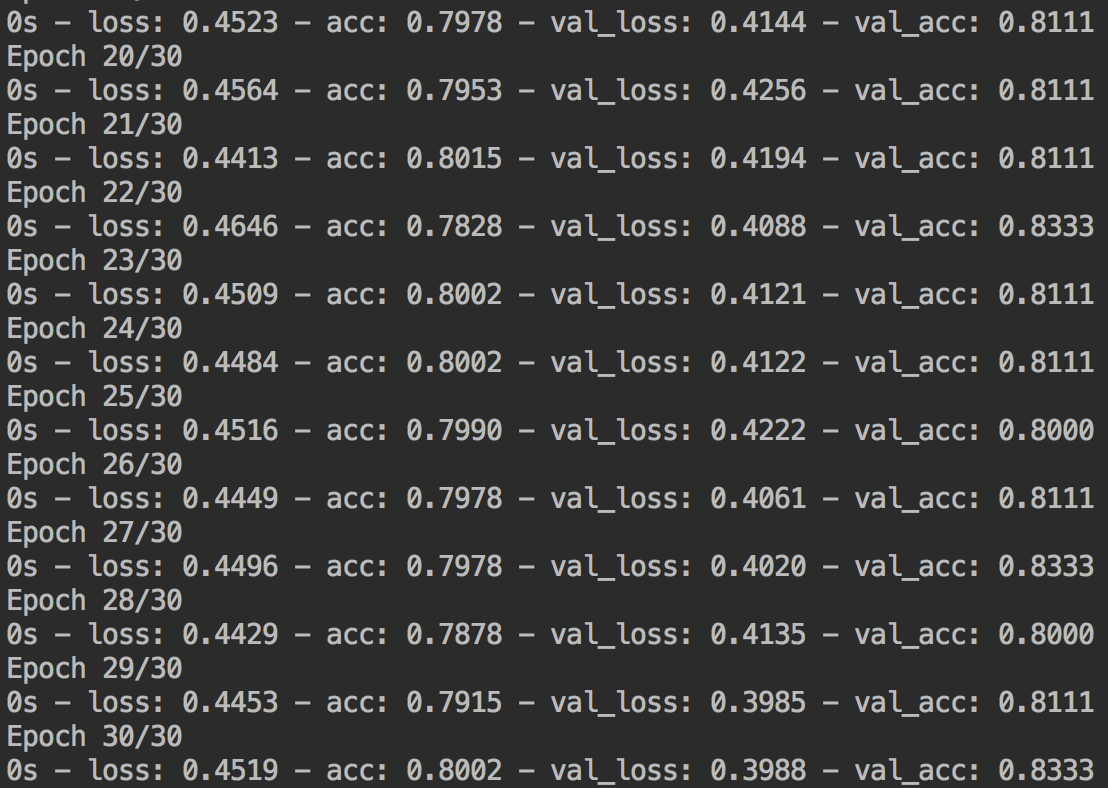
\includegraphics[width=1.0\textwidth]{image/acc.png}
\end{figure}

\newpage
\section{Evaluation}
最後,把準確率畫出來,並計算成效

\begin{shaded}
\begin{lstlisting}[language=Python]
import matplotlib.pyplot as plt

def get_evaluate():
  scores = model.evaluate(
  		x=np.array(x_test), 
  		y=np.array(y_test))

def show_train_history(train_history, train, val):
  plt.plot(train_history.history[train])
  plt.plot(train_history.history[validation])
  plt.title('Train History')
  plt.ylabel('Train')
  plt.xlabel('Epoch')
  plt.legend(['train', 'validation'], 
  			loc ='center right')
  plt.show()
\end{lstlisting}
\end{shaded}

\begin{figure}[ht]
\centering
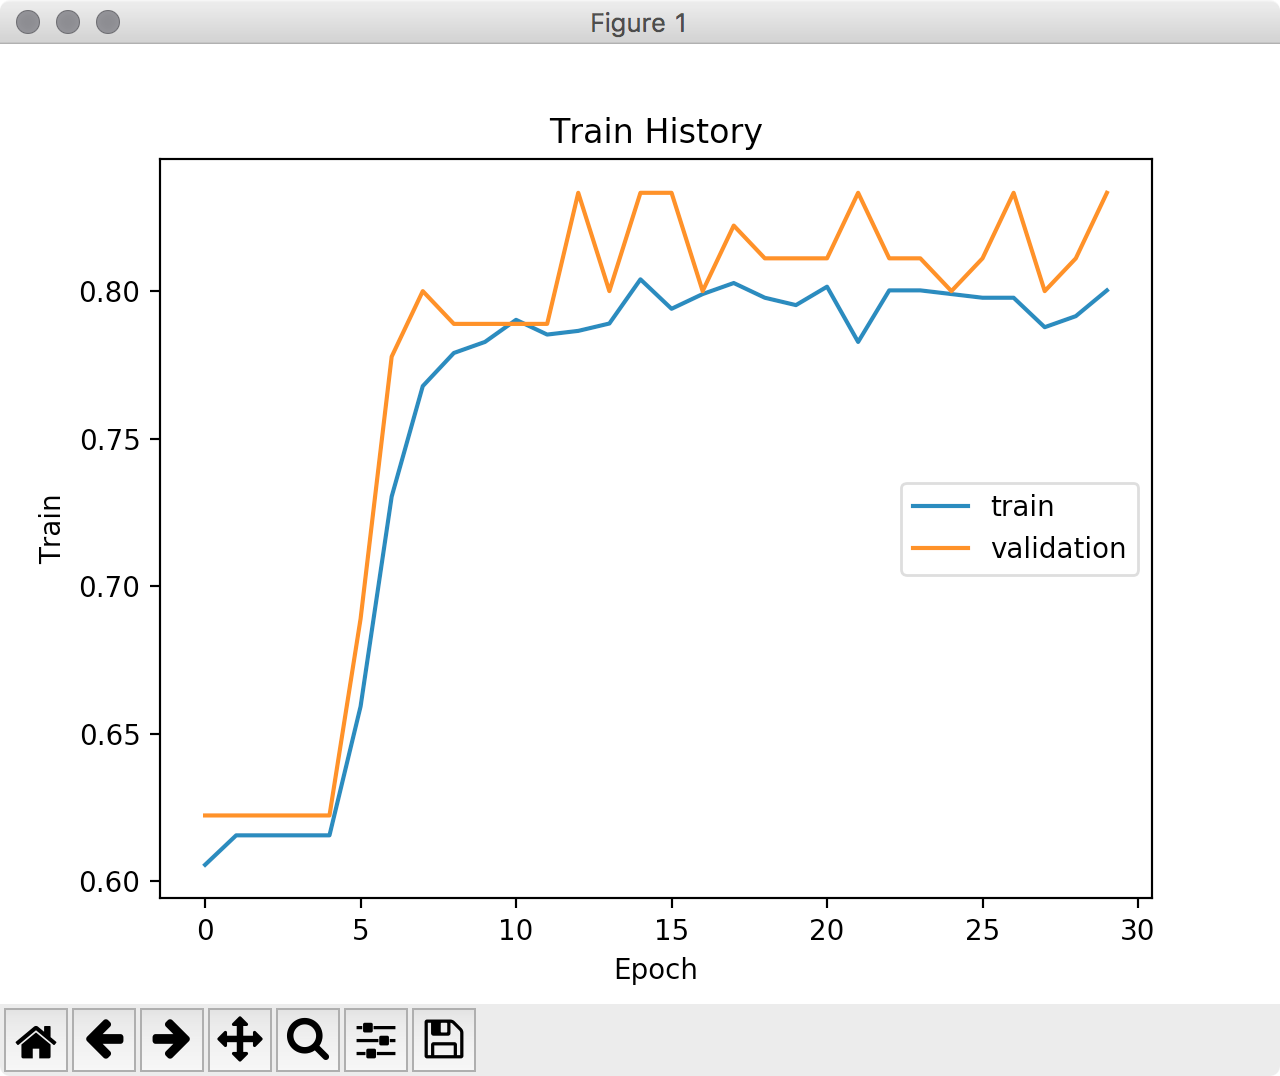
\includegraphics[width=0.8\textwidth]{image/result.png}
\end{figure}

\end{document}